% SC4013 --- Chapter 6: Cryptographic Misuse in Applications (0->100 ground-up)
\chapter{Cryptographic Misuse in Applications}
\label{ch:crypto-app}

\begin{quote}
\emph{``Crypto rarely fails because the math is wrong; it fails because the code calls it wrong.''} --- JWTs, password hashes and random numbers look simple. Each has a misuse that voids the guarantee silently.
\end{quote}

\noindent\fbox{\parbox{\dimexpr\linewidth-2\fboxsep-2\fboxrule}{%
\textbf{From zero: what app crypto must do.} We assume no prior crypto beyond ``encryption hides data.'' We build from password storage to tokens to randomness, showing why correct primitives with wrong parameters are as bad as no crypto.}}
\vspace{0.4em}

\section*{Learning Outcomes}
After this chapter you will be able to:
\begin{enumerate}[label=(L\arabic*)]
    \item explain why fast hashes (SHA-256, MD5) are wrong for passwords;
    \item compare bcrypt, scrypt and Argon2 and choose parameters;
    \item dissect a JWT, list its misuse classes, and validate one securely;
    \item identify weak randomness, hard-coded secrets and IV/nonce reuse;
    \item apply AEAD and key-management best practices in application code.
\end{enumerate}

% ============================================================
\section{Password Hashing: Slow Is a Feature}
\label{sec:pw-hashing}
Storing passwords as plaintext or fast hashes (MD5, SHA-1, SHA-256) lets an attacker who leaks the DB test billions of guesses per second on a GPU. Password hashing must be \emph{slow, salted and memory-hard}.

\begin{description}[leftmargin=1.2em,itemsep=0.30em]
    \item[Salt] A 16-byte random per-user value so identical passwords hash differently and rainbow tables fail. Stored alongside the hash; not secret.
    \item[Work factor] Tunable cost (iterations, time, memory) so hashing takes $\sim$100\,ms today and scales as hardware improves.
    \item[Memory hardness] Forces the attacker to use memory per guess, blunting GPU/ASIC parallelism. Argon2id and scrypt have it; bcrypt partially.
\end{description}

\begin{figure}[h]\centering
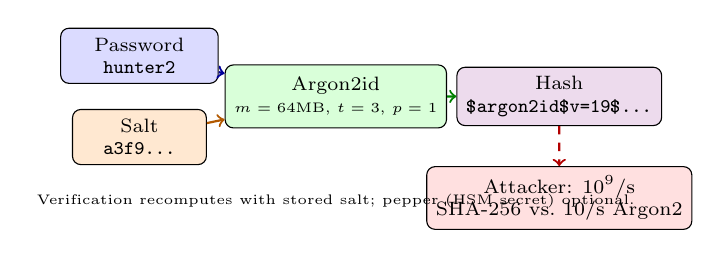
\begin{tikzpicture}[scale=0.86,every node/.style={font=\scriptsize}]
  \node[draw,fill=blue!14,rounded corners=3pt,minimum width=2.0cm,minimum height=0.7cm,align=center] (pw) at (-4.2,1.6) {Password\\\texttt{hunter2}};
  \node[draw,fill=orange!18,rounded corners=3pt,minimum width=1.7cm,minimum height=0.7cm,align=center] (salt) at (-4.2,0.4) {Salt\\\texttt{a3f9...}};
  \node[draw,fill=green!15,rounded corners=3pt,minimum width=2.4cm,minimum height=0.8cm,align=center] (kdf) at (-1.3,1.0) {Argon2id\\\tiny $m=64$MB, $t=3$, $p=1$};
  \node[draw,fill=violet!14,rounded corners=3pt,minimum width=2.6cm,minimum height=0.7cm,align=center] (out) at (2.0,1.0) {Hash\\{\scriptsize \texttt{\$argon2id\$v=19\$...}}};
  \node[draw,fill=red!12,rounded corners=3pt,minimum width=2.2cm,minimum height=0.7cm,align=center] (atk) at (2.0,-0.5) {Attacker: $10^9$/s\\SHA-256 vs.\ $10$/s Argon2};
  \draw[->,thick,blue!60!black] (pw) -- (kdf);
  \draw[->,thick,orange!70!black] (salt) -- (kdf);
  \draw[->,thick,green!50!black] (kdf) -- (out);
  \draw[->,thick,red!70!black,dashed] (out) -- (atk);
  \node[font=\tiny,align=center] at (-1.3,-0.55) {Verification recomputes with stored salt; pepper (HSM secret) optional.};
\end{tikzpicture}
\caption{Password hashing with salt and a memory-hard KDF. The same password yields different stored strings; verification is deliberately slow.}
\label{fig:pw-kdf}
\end{figure}

Why not SHA-256? A GPU does $\sim 10^9$ SHA-256/s vs.\ $\sim 10$ Argon2id/s with $64$\,MB. A 8-char password falls in hours vs.\ millennia. Pepper (a secret stored in an HSM, mixed as \texttt{HMAC(pepper, salt||pw)}) adds defence if the DB alone leaks.

\begin{lstlisting}[language=Python]
# CORRECT: Argon2id with per-user salt (argon2-cffi)
from argon2 import PasswordHasher
ph = PasswordHasher(time_cost=3, memory_cost=65536, parallelism=1)  # 64 MB
stored = ph.hash("hunter2")          # generates random salt internally
ph.verify(stored, "hunter2")         # True; raises on mismatch
# WRONG: fast hash, no salt, no pepper
import hashlib
bad = hashlib.sha256(b"hunter2").hexdigest()  # GPU-crackable; never do this
\end{lstlisting}

Params: bcrypt cost 10--12, Argon2id $m\ge 64$\,MB, $t\ge 3$ for interactive logins; re-hash on login if stored params are weaker than current policy. Never cap password length below 64; normalise Unicode (NFKC) first.

% ============================================================
\section{JWT: A Token That Must Be Verified, Not Just Read}
\label{sec:jwt}
A JSON Web Token is \texttt{header.payload.signature} (base64url). Header says \texttt{alg} (e.g., HS256, RS256); payload carries claims (\texttt{sub}, \texttt{exp}, \texttt{aud}, \texttt{iss}); signature is \texttt{Sign(key, header.payload)}. Stateless auth is the appeal; the pitfall is trusting the token without verifying it exactly as the issuer did.

Misuse classes:
\begin{description}[leftmargin=1.2em,itemsep=0.30em]
    \item[\texttt{alg:none}] Server accepts unsigned tokens if the library is configured to allow it.
    \item[Algorithm confusion] Attacker sends RS256 token signed with HS256 using the RSA public key as the HMAC secret.
    \item[Weak HS256 secret] Short or guessable secret brute-forced offline.
    \item[Missing claim checks] \texttt{exp}, \texttt{aud}, \texttt{iss}, \texttt{nbf} not checked; stolen or cross-service tokens replay.
    \item[\texttt{kid} traversal] \texttt{kid} used as a file path (\texttt{../../dev/null}) or SQL lookup without sanitising.
\end{description}

\begin{figure}[h]\centering
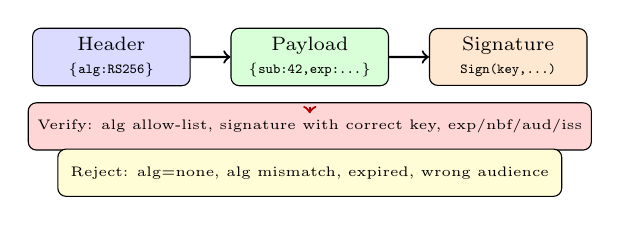
\begin{tikzpicture}[scale=0.84,every node/.style={font=\scriptsize}]
  \node[draw,fill=blue!14,rounded corners=3pt,minimum width=2.0cm,minimum height=0.7cm,align=center] (hdr) at (-3.6,1.4) {Header\\\tiny \texttt{\{alg:RS256\}}};
  \node[draw,fill=green!15,rounded corners=3pt,minimum width=2.0cm,minimum height=0.7cm,align=center] (pay) at (-0.6,1.4) {Payload\\\tiny \texttt{\{sub:42,exp:...\}}};
  \node[draw,fill=orange!18,rounded corners=3pt,minimum width=2.0cm,minimum height=0.7cm,align=center] (sig) at (2.4,1.4) {Signature\\\tiny \texttt{Sign(key,...)}};
  \draw[->,thick] (hdr) -- (pay); \draw[->,thick] (pay) -- (sig);
  \node[draw,fill=red!16,rounded corners=3pt,minimum width=6.4cm,minimum height=0.6cm,align=center,font=\tiny] at (-0.6,0.35) {Verify: alg allow-list, signature with correct key, exp/nbf/aud/iss};
  \node[draw,fill=yellow!16,rounded corners=3pt,minimum width=6.4cm,minimum height=0.6cm,align=center,font=\tiny] at (-0.6,-0.35) {Reject: alg=none, alg mismatch, expired, wrong audience};
  \draw[->,thick,red!70!black] (-0.6,0.65) -- (-0.6,0.55);
\end{tikzpicture}
\caption{JWT structure and the verification checklist. Every field outside the signature is attacker-controlled; only the signature binds it.}
\label{fig:jwt-verify}
\end{figure}

\begin{lstlisting}[language=Python]
# SECURE JWT verification (PyJWT) -- allow-list alg, check claims
import jwt
payload = jwt.decode(token,
    key=RSA_PUBLIC_KEY,            # RS256: public key; HS256: strong random 256-bit secret
    algorithms=["RS256"],          # never ["none"] and never attacker-chosen
    audience="my-api", issuer="auth.example.com",
    options={"require": ["exp","aud","iss"]})
# Insecure patterns: algorithms=["none"], verify_signature=False,
#   or algorithms from header (jwt.get_unverified_header(token)["alg"])
\end{lstlisting}

Use short expiry (5--15\,min) plus refresh tokens stored httpOnly+Secure+SameSite. Prefer opaque session IDs or PASETO/Branca if you do not need third-party verification; JWT is not encryption (use JWE if confidentiality is needed).

% ============================================================
\section{Randomness, Secrets and AEAD Misuse}
\label{sec:random-aead}
\begin{description}[leftmargin=1.2em,itemsep=0.30em]
    \item[Randomness] \texttt{Math.random()}, \texttt{rand()}, or \texttt{random} are predictable. Use \texttt{os.urandom} / \texttt{getrandom} / \texttt{CSPRNG}. Nonce/IV must never repeat for a key (AES-GCM fails catastrophically on reuse).
    \item[Hard-coded secrets] API keys in GitHub, baked into APKs, or in client JS are public. Store in a vault/KMS, rotate, scope narrowly.
    \item[ECB and unauthenticated CBC] ECB leaks patterns; CBC without MAC leaks padding oracles. Use AEAD: AES-GCM or ChaCha20-Poly1305 via a high-level library.
    \item[Key management] Never derive a key by truncating a password; use the KDF above. Separate keys per purpose (enc vs.\ MAC) and rotate with versioned key IDs.
\end{description}

\begin{figure}[h]\centering
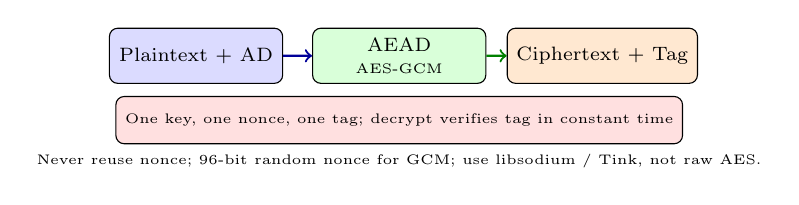
\begin{tikzpicture}[scale=0.86,every node/.style={font=\scriptsize}]
  \node[draw,fill=blue!14,rounded corners=3pt,minimum width=2.2cm,minimum height=0.7cm,align=center] (pt) at (-3.8,1.2) {Plaintext + AD};
  \node[draw,fill=green!15,rounded corners=3pt,minimum width=2.2cm,minimum height=0.7cm,align=center] (aead) at (-0.8,1.2) {AEAD\\\tiny AES-GCM};
  \node[draw,fill=orange!18,rounded corners=3pt,minimum width=2.0cm,minimum height=0.7cm,align=center] (ct) at (2.2,1.2) {Ciphertext + Tag};
  \draw[->,thick,blue!60!black] (pt) -- (aead);
  \draw[->,thick,green!50!black] (aead) -- (ct);
  \node[draw,fill=red!12,rounded corners=3pt,minimum width=5.8cm,minimum height=0.6cm,align=center,font=\tiny] at (-0.8,0.25) {One key, one nonce, one tag; decrypt verifies tag in constant time};
  \node[font=\tiny,align=center] at (-0.8,-0.35) {Never reuse nonce; 96-bit random nonce for GCM; use libsodium / Tink, not raw AES.};
\end{tikzpicture}
\caption{AEAD as the safe default. Associated data (headers, IDs) is authenticated but not encrypted; tampering is detected via the tag.}
\label{fig:aead}
\end{figure}

Prefer high-level libraries (libsodium, Google Tink, Fernet) over raw primitives. They pick nonces, handle padding, and fail closed (one generic error, constant-time comparison).

% ============================================================
\section{Secrets Management and Key Rotation}
\label{sec:secrets-mgmt}
A secret that lives in a repo is not a secret. Threat: Git history retains it forever; forks and CI logs copy it; APKs and JS bundles ship it to every user. Manage secrets with a vault (HashiCorp Vault, AWS Secrets Manager, GCP Secret Manager) or KMS/HSM. App fetches at startup, never from env files committed to Git. Scan repos with Gitleaks/TruffleHog in pre-commit and CI; block push if a high-entropy string matches an API-key pattern.

Key rotation: version keys (\texttt{key\_id} in JWT header or DB), keep old keys for verification/decryption, new keys for signing/encryption. Rotate on a calendar (90 days) and on incident (revoke immediately). Key derivation: use HKDF to derive purpose-bound subkeys from a master: \texttt{K\_enc = HKDF(master, "enc-v1")}, \texttt{K\_mac = HKDF(master, "mac-v1")} so a leak of one does not compromise the other.

\begin{example}[Kid traversal to RCE]
Server does \texttt{key = open("/keys/" + kid).read()} where \texttt{kid} comes from the JWT header. Attacker sends \texttt{kid=../../etc/passwd} or \texttt{kid=../../dev/null} or a path to an attacker-controlled file. Fix: map \texttt{kid} through an allow-list dictionary, never concatenate into a path; load keys by \texttt{key\_id} lookup, not filesystem access.
\end{example}

\begin{remark}[Pepper vs.\ salt]
Salt is per-user, stored with the hash, not secret. Pepper is a short secret ($32$ bytes) stored in an HSM, applied as \texttt{HMAC(pepper, salt||pw)} before the KDF. If the DB leaks but the HSM does not, the attacker still cannot crack without the pepper. Rotate pepper by storing \texttt{pepper\_id} alongside the hash; verify with the old pepper, re-hash with the new on login.
\end{remark}

\begin{example}[Insecure randomness in session IDs]
\texttt{session\_id = str(randint(0, 2**31))} has 31 bits of entropy; an attacker enumerates it in seconds. Use \texttt{secrets.token\_urlsafe(32)} (256 bits from the CSPRNG) and store only a SHA-256 of the token in the DB (so a DB leak does not give live sessions).
\end{example}

\subsection{TLS and At-Rest Encryption Checklist}
For TLS: prefer TLS~1.3, AEAD ciphers (AES-GCM, ChaCha20-Poly1305), disable TLS~1.0/1.1, pin with HSTS (\texttt{Strict-Transport-Security: max-age=31536000; includeSubDomains}), and verify certificates (never \texttt{verify=False}). For data at rest: encrypt columns containing PII with AEAD, use envelope encryption (DEK per record, KEK in KMS), and never log plaintext. Validate with \texttt{testssl.sh} and a scanner like \texttt{cryptolyzer}.

\begin{remark}[Don't roll your own crypto]
If you are writing \texttt{AES\_encrypt} directly, you are probably missing authentication, padding, nonce management, and constant-time comparison. Use Fernet (\texttt{cryptography.fernet}), NaCl \texttt{crypto\_secretbox}, or Tink \texttt{Aead}; they compose correctly and fail closed.
\end{remark}

\subsection{Migration Path for Legacy Hashes}
Legacy DBs often contain MD5 or unsalted SHA-1. Migrate without forcing a global reset: on login, if \texttt{algo != "argon2id"} verify against the old hash, then immediately \texttt{ph.hash(password)} and overwrite the stored value, tagging it \texttt{argon2id}. Over weeks the table converges. For users who never log in, force a reset after a grace window and expire old hashes. Never ``wrap'' a fast hash as \texttt{argon2id(md5(pw))} without also re-hashing on next login; the inner MD5 is still fast to brute-force offline if the outer layer is leaked.

\begin{example}[Timing side channel in comparison]
\texttt{if user\_hash == computed:} leaks timing (Python \texttt{==} short-circuits). Use \texttt{hmac.compare\_digest} or \texttt{secrets.compare\_digest} for constant-time comparison, though Argon2 verify already does. For JWT signatures and HMAC checks, constant-time is mandatory; a 10\,ms timing difference over the network has been used to forge tags.
\end{example}

\subsection{TLS and At-Rest: Putting Keys to Work}
Envelope encryption separates the data-encryption key (DEK, per record or per table) from the key-encryption key (KEK, in KMS). The DEK encrypts the data; the KEK encrypts the DEK. Rotating the KEK only re-encrypts DEKs, not all data, which makes frequent rotation practical. On AWS this is \texttt{GenerateDataKey} + \texttt{Encrypt}; on GCP it is \texttt{DEK = AEAD(KMS\_key, plaintext)}.

For mobile and SPA clients, never ship a long-lived secret. Issue short-lived tokens via an exchange endpoint that authenticates the app (attestation, mTLS, or device check) and logs the grant. This confines a leaked binary to a small window and gives the server a revocation point.

\begin{remark}[Compliance mapping]
OWASP ASVS 6.2, NIST 800-63B and PCI DSS all require memory-hard password hashing, unique salts, and pepper or HSM-backed secrets. Auditors will ask for the algorithm, parameters ($m,t,p$), salt length, and rotation evidence---keep them in a runbook, not just in code.
\end{remark}

\begin{example}[Audit checklist: what to demand in review]
A reviewer should verify: (i)~\texttt{argon2} or \texttt{bcrypt} with current params, (ii)~no raw SHA/MD5 for passwords, (iii)~JWT allow-list + claim checks + short expiry, (iv)~CSPRNG for tokens/nonces, (v)~AEAD with no nonce reuse, (vi)~no secret in repo/APK/JS, (vii)~vault/KMS + rotation. A single ``use SHA-256 with salt'' comment in a PR should block merge.
\end{example}

\begin{remark}[Session vs.\ JWT trade-off]
Opaque sessions (random ID $\to$ server-side store) are revocable instantly but require a lookup. JWTs are stateless but revocation is harder (blocklist or short expiry). Choose sessions for first-party web apps, JWTs for microservice-to-microservice or third-party delegation where stateless verification matters. Hybrid: JWT for 5\,min, refresh via opaque rotation.
\end{remark}

\begin{remark}[Crypto agility]
Algorithms age. Store \texttt{alg} and \texttt{version} with every encrypted value and hash so you can migrate without re-encrypting everything at once. Crypto agility---the ability to switch primitives without a flag day---is an OWASP ASVS requirement and a practical necessity when a cipher is deprecated.
\end{remark}

% ============================================================
\section{Exercises}
\label{sec:ch05-exercises}
\begin{enumerate}[label=E5.\arabic*, leftmargin=*, itemsep=0.6em]
    \item \textbf{Password audit.} A DB uses \texttt{SHA256(salt||pw)} with 8-byte salts and no work factor. Estimate GPU guesses/sec vs.\ Argon2id ($64$\,MB, $t=3$). Propose a migration that re-hashes on next login without forcing a reset.
    \item \textbf{JWT confusion.} Explain the RS256$\to$HS256 confusion: what the attacker sends, why \texttt{HMAC(public\_key, data)} verifies if the server picks HS256 from the header, and the one-line fix (allow-list).
    \item \textbf{None and kid.} Write two malicious JWTs: one with \texttt{alg:none} and one where \texttt{kid=../../etc/passwd}. State the server-side check that blocks each and the error returned.
    \item \textbf{Nonce reuse.} AES-GCM encrypts two messages $m_1,m_2$ with the same key+nonce. Show what an attacker learns from $c_1 \oplus c_2$. How does a 96-bit random nonce with a counter avoid this? When would you use deterministic SIV instead?
    \item \textbf{Secret in the APK.} A mobile app ships with \texttt{API\_KEY="sk-live-..."} in the binary. Describe extraction (JADX/strings), impact, and a fix using short-lived tokens via an exchange endpoint with attestation.
\end{enumerate}

\section*{Chapter Notes}
Password hashing guidance follows NIST SP 800-63B and the Password Hashing Competition (Argon2, 2015). JWT misuses are catalogued in RFC 8725 and ``Critical vulnerabilities in JWT'' (Sakuragi et al.); algorithm confusion was described by Tim McLean (2015). AEAD and nonce guidance follows RFC 5116 and libsodium/Tink docs; randomness failures are surveyed in Heninger et al.\ (2012) on weak keys.

% End of Chapter 6
